\newcommand{\meanPerSampleScores}{
    \begin{table}[H]
        \centering
        \begin{tabular}{|p{3,2cm}||p{1,8cm} p{1,8cm} p{1,8cm} p{1,8cm} p{1,8cm}|}
            \hline
            Mean per-sample & \multicolumn{5}{c|}{\textbf{FPR}} \\
            tagging scores & $10^{-5}$ & $10^{-4}$ & $10^{-3}$ & $10^{-2}$ & $10^{-1}$ \\
            \hline
            \multicolumn{6}{|c|}{\textbf{Jaccard Similarity}} \\
            \hline
            ALOHA & 0.719$\pm$0.001 & 0.719$\pm$0.001 & 0.719$\pm$0.000 & \textBF{0.711$\pm$0.002} & \textBF{0.512$\pm$0.044} \\
            Joint Embedding & \textBF{0.724$\pm$0.002} & \textBF{0.724$\pm$0.002} & 0.724$\pm$0.002 & 0.702$\pm$0.003 & 0.362$\pm$0.008 \\
            Proposed Model & 0.723$\pm$0.001 & 0.723$\pm$0.001 & \textBF{0.726$\pm$0.001} & 0.707$\pm$0.006 & 0.417$\pm$0.061 \\
            \hline
            \multicolumn{6}{|c|}{\textbf{Mean per-Sample Accuracy}} \\
            \hline
            ALOHA & 0.718$\pm$0.000 & 0.718$\pm$0.000 & 0.718$\pm$0.001 & \textBF{0.705$\pm$0.001} & \textBF{0.494$\pm$0.049} \\
            Joint Embedding & \textBF{0.722$\pm$0.000} & \textBF{0.722$\pm$0.000} & 0.719$\pm$0.002 & 0.687$\pm$0.006 & 0.326$\pm$0.010 \\
            Proposed Model & 0.720$\pm$0.002 & 0.720$\pm$0.002 & \textBF{0.720$\pm$0.003} & 0.694$\pm$0.009 & 0.384$\pm$0.066 \\
            \hline
        \end{tabular}
        \caption{Mean and standard deviation of mean per-sample tagging results (\textit{Jaccard simialrity} and \textit{mean per-sample accuracy}) for the different models. Results were aggregated over \textBF{3} training runs with different weight initializations and minibatch orderings. Best results are shown in \textbf{bold}.} \label{tab:meanPerSampleScores}
    \end{table}
}

\newcommand{\allMeanRocAloha}{
    \begin{figure}[H]
        \vspace*{-0.5cm}
        \centering
        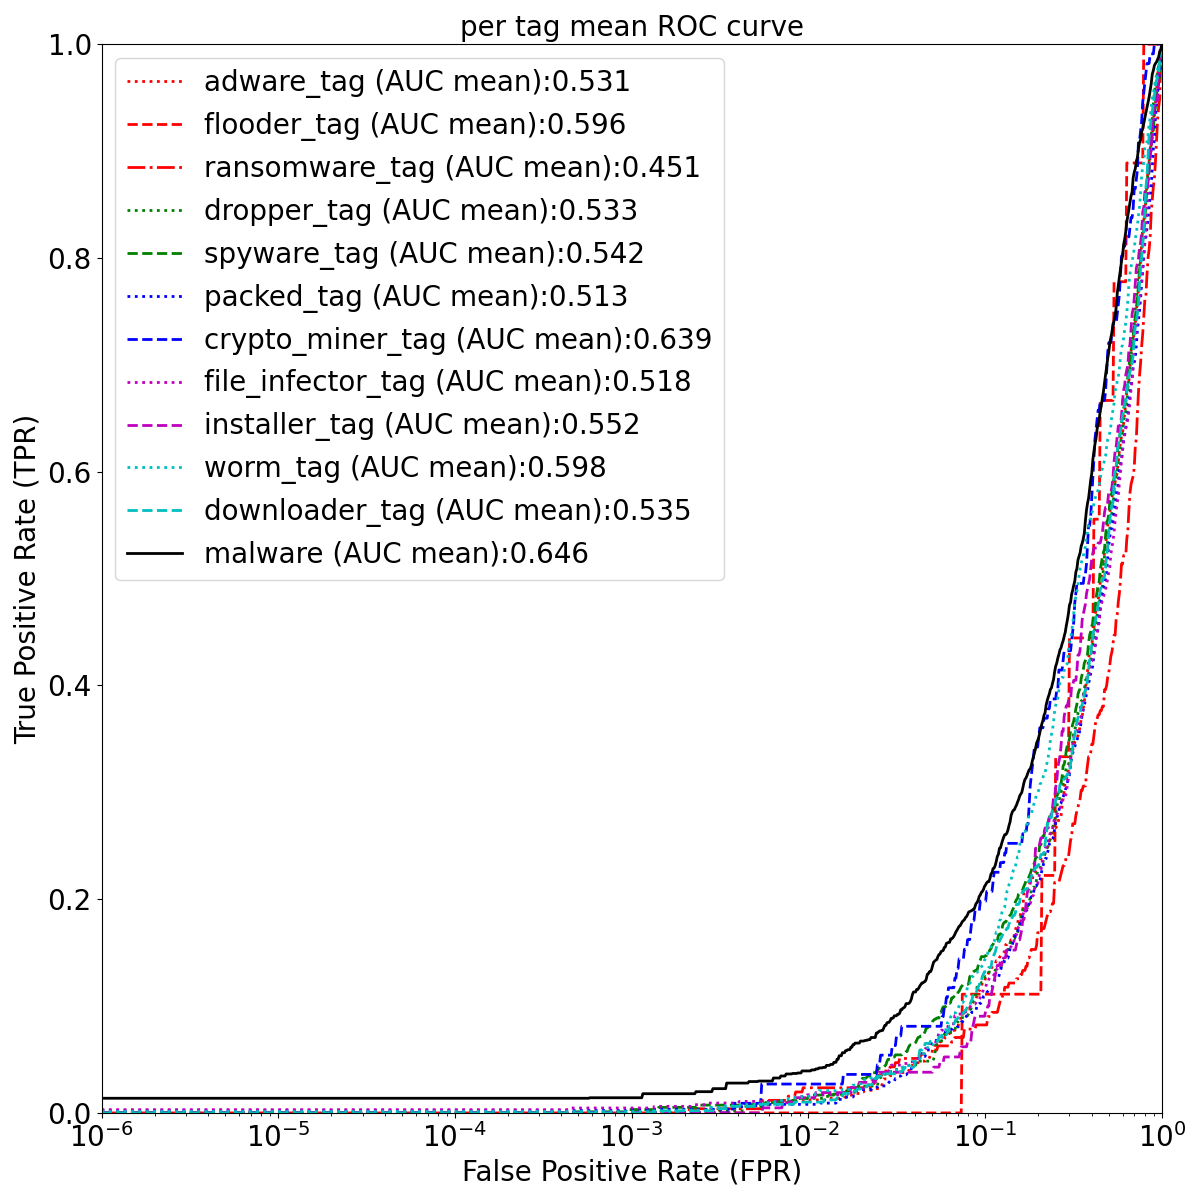
\includegraphics[width=0.6\textwidth]{./results/all_mean_roc_aloha.png}
        \vspace*{-0.2cm}
        \caption{Mean ROC curve and AUC statistics of \textBF{ALOHA} model for the tags/labels. The line represents the \textit{mean} TPR at a given FPR. Statistics were computed over \textBF{3} training runs, each with random parameter initialization.}
        \label{fig:allMeanRocAloha}
    \end{figure}
}

\newcommand{\allMeanRocJointEmbedding}{
    \begin{figure}[H]
        \vspace*{-0.5cm}
        \centering
        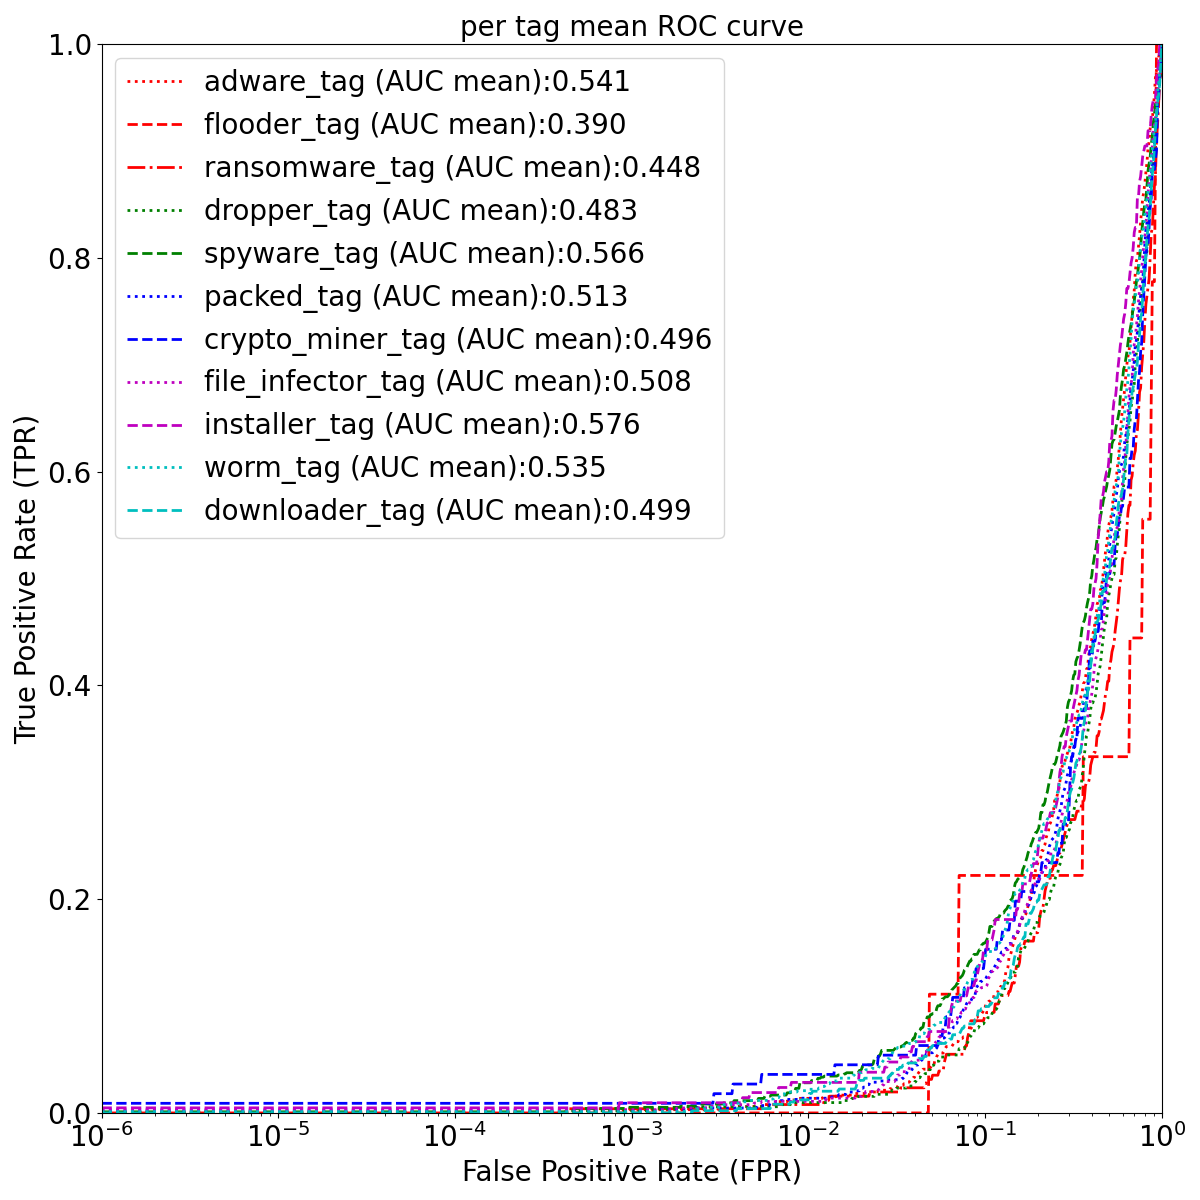
\includegraphics[width=0.6\textwidth]{./results/all_mean_roc_jointEmbedding.png}
        \vspace*{-0.2cm}
        \caption{Mean ROC curve and AUC statistics of \textBF{Joint Embedding} model for all tags/labels. The line represents the \textit{mean} TPR at a given FPR. Statistics were computed over \textBF{3} training runs, each with random parameter initialization.}
        \label{fig:allMeanRocJointEmbedding}
    \end{figure}
}

\newcommand{\allMeanRocProposedModel}{
    \begin{figure}[H]
        \vspace*{-0.5cm}
        \centering
        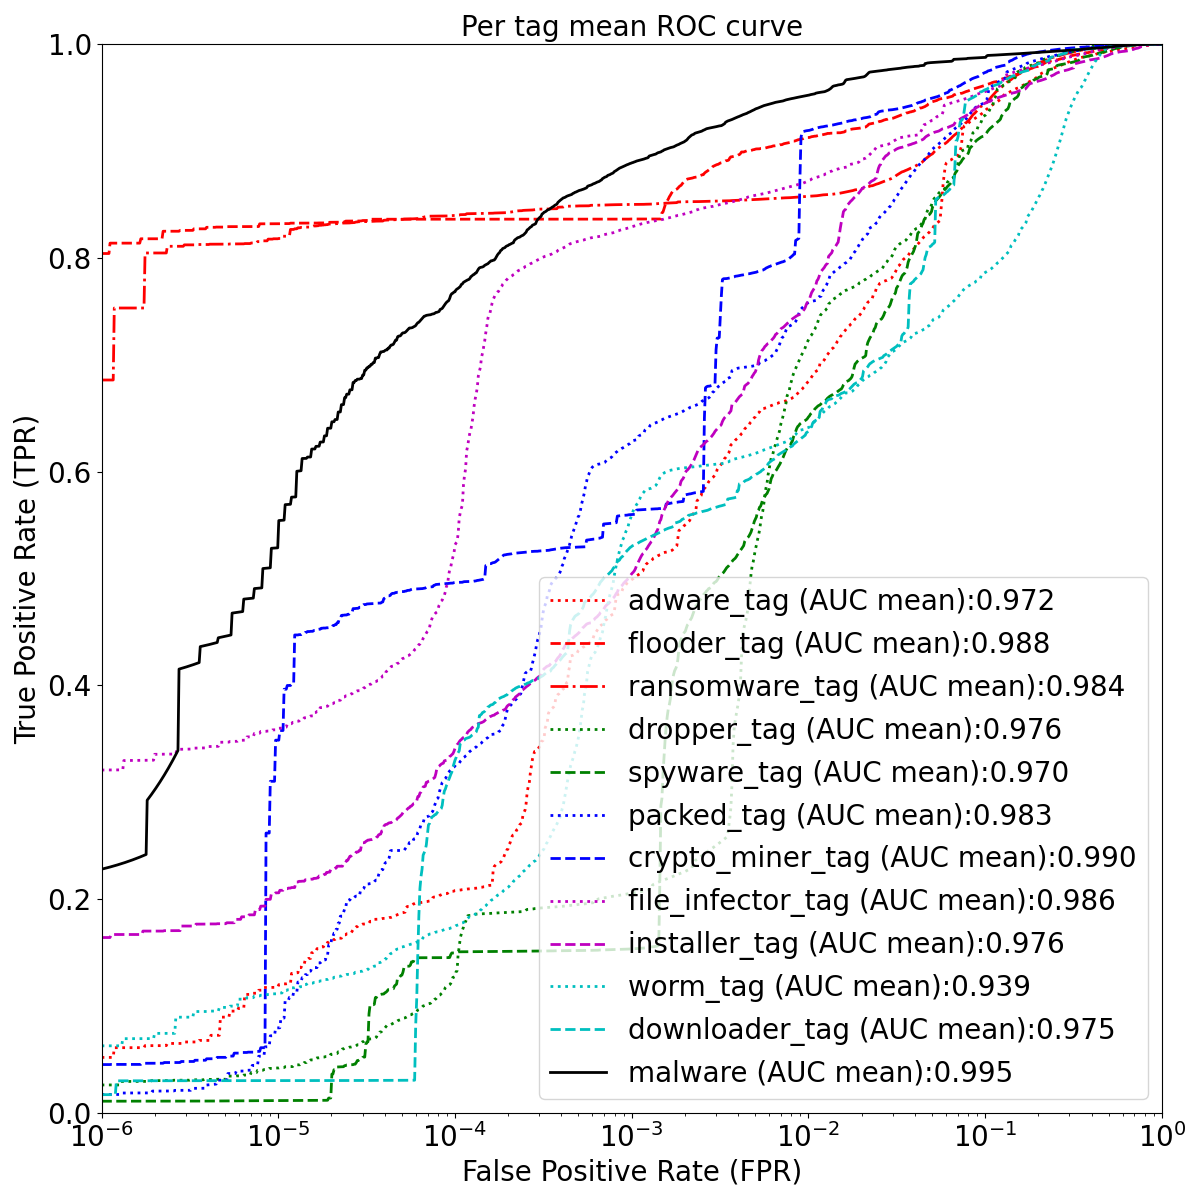
\includegraphics[width=0.6\textwidth]{./results/all_mean_roc_proposedModel.png}
        \vspace*{-0.2cm}
        \caption{Mean ROC curve and AUC statistics of \textBF{Proposed Model} for the tags/labels. The line represents the \textit{mean} TPR at a given FPR. Statistics were computed over \textBF{3} training runs, each with random parameter initialization.}
        \label{fig:allMeanRocProposedModel}
    \end{figure}
}